%% ****** Start of file aiptemplate.tex ****** %
%%
%%   This file is part of the files in the distribution of AIP substyles for REVTeX4.
%%   Version 4.1 of 9 October 2009.
%%
%
% This is a template for producing documents for use with 
% the REVTEX 4.1 document class and the AIP substyles.
% 


\documentclass[aip,graphicx]{revtex4-1}
\usepackage{graphicx}
\usepackage{longtable}
\usepackage[version=3]{mhchem} % Formula subscripts using \ce{}
\usepackage[T1]{fontenc}       % Use modern font encodings
\usepackage{amsmath}
\usepackage[dvipsnames]{xcolor}
% NB added command for in line cite
%\newcommand{\onlinecite}[1]{\hspace{-1 ex} \nocite{#1}\citenum{#1}} 
%\documentclass[aip,reprint]{revtex4-1}

\draft % marks overfull lines with a black rule on the right

\begin{document}

% Use the \preprint command to place your local institutional report number 
% on the title page in preprint mode.
% Multiple \preprint commands are allowed.
%\preprint{}

\title{Velocity Map Imaging Spectroscopy of C$_2$H$^-$ and C$_2$D$^-$: a benchmark study of vibronic coupling interactions}


\author{Benjamin~A.~Laws}
\email{b.laws@unsw.edu.au}
\affiliation{School of Chemistry, University of New South Wales, Sydney NSW 2052, Australia}
\affiliation{Research School of Physics, The Australian
	National University, Canberra ACT 2601, Australia}
\author{Zachariah~D.~Levey} 
\affiliation{School of Chemistry, University of New South Wales, Sydney NSW 2052, Australia}
\author{Andrei Sanov}
\affiliation{Department of Chemistry and Biochemistry, The University of Arizona, Tucson, Arizona 85721, United States}
\author{John F. Stanton}
\affiliation{Department of Chemistry, University of Florida, Gainesville, Florida 32611, United States}
\author{Timothy~W.~Schmidt} 
\affiliation{School of Chemistry, University of New South Wales, Sydney NSW 2052, Australia}
\author{Stephen~T.~Gibson}
\affiliation{Research School of Physics, The Australian
	National University, Canberra ACT 2601, Australia}




\date{\today}

\begin{abstract}
High-resolution velocity-map imaged photoelectron spectra of the ethynyl anions C$_2$H$^-$ and C$_2$D$^-$ are measured over a range of photodetachment wavelengths, to investigate the complex interactions between the close lying $\tilde{X}^2\Sigma^+$ and $\tilde{A}^2\Pi$ electronic states. Vibronic coupling calculations are performed by transforming to a quasidiabatic representation, parametrised by \emph{ab-initio} CFOUR calculations, to model the interplay between pseudo Jahn-Teller and Renner-Teller coupling. This approach is combined with electron anisotropy measurements to assign all of the observed vibronic structure, providing a framework that may be used to accurately simulate spectra of larger C$_{2n}$H monohydride carbon chains.
\end{abstract}

\pacs{}

\maketitle 

\section{Introduction}
Carbon monohydrides C$_{2n}$H, are a class of linear radicals that play an important role in combustion and interstellar chemistry~\cite{kie90,kie92,bou96,wil91,vui01}. These carbon chains have been observed in many interstellar environments, including planetary atmospheres~\cite{vui01,wil03,dob16}, comets~\cite{jac96}, dark clouds~\cite{ziu82,gup09}, and during heavy star formation~\cite{beu08,jia15}. Due to their relatively high abundance in a variety of astronomical conditions, they are believed to be promising candidates for Diffuse Interstellar Band (DIB) carriers~\cite{dou77,ful93,wat94,ful00,sch05,gup09}. The corresponding anions C$_{2n}$H$^-$ are also believed to play an important role in interstellar chemistry~\cite{mil17,gup09}. C$_6$H$^-$ was the first negative ion detected in space, after it was observed in two distinct interstellar molecular clouds IRC+10216 and TMC-1 in 2006~\cite{mcc06}. More recently, anions C$_4$H$^-$~\cite{cer07} and C$_8$H$^-$~\cite{bru07,rem07} have also been detected in a range of environments, include dark clouds~\cite{cor13}, prestellar cores,~\cite{sak10} and prostellar envelopes~\cite{sak07}.

Chain growth of the C$_{2n}$H radicals occurs predominately through acetylene addition,~\cite{wil03}
\begin{equation}
\text{C}_{2n}\text{H} + \text{C}_2\text{H}_2 \rightarrow \text{C}_{2n+2}\text{H}+\text{H}_2.
\end{equation}
Conversely, the formation of anions in space is believed to be driven by radiative electron attachment, charge transfer, and dissociative electron attachment. Current astrochemical modelling of interstellar clouds, such as IRC+10216, typically underestimate the observed abundances of CH$_4^-$~\cite{mil17,cor13,her08}. Therefore, it has been proposed that ion-neutral reactions
\begin{equation}
\text{C}_{2n}\text{H}^- + \text{C}_2\text{H}_2 \rightarrow \text{C}_{2n+2}\text{H}^- + \text{H}_2.
\end{equation}
may be significant chain growth mechanisms that also needs to be included in astrochemical models~\cite{mil17,bas19}. Studies of the extraterrestrial planetary atmosphere of Saturn's moon Titan suggest that both C$_2$H and C$_2$H$^-$ play an important role in the atmospheric chemistry~\cite{dob16,vui09,des17,vri18}. Multiple reaction pathways involving the C$_2$H$^-$ have been proposed, including reactions with C$_2$H$_2$ and HCN. 

Our knowledge of interstellar chemistry relies critically on theory, to provide a link between astronomical observations and terrestrial laboratory studies. Microwave spectroscopy has successfully been used in this fashion to identify a large number of molecules in the interstellar medium (ISM). However for some species, particularly those with low abundances or no dipole moment, UV/vis spectroscopic methods are required for identification~\cite{mai97}. This creates a challenge for theory, as electronic spectral calculations are more difficult than those employed for pure rotational spectra~\cite{for10}. This becomes even more challenging when vibronic coupling effects are introduced, as they can be exceedingly difficult to model.

These considerations may be explored by examining some of the smallest carbon monohydrides. The ethynyl radical C$_2$H may appear to be a simple linear triatomic molecule. However the electronic spectrum is complicated by the presence of the close-lying ground $^2\Sigma^+$ and first excited $^2\Pi$ surfaces, which are only separated by $\sim3,700~$cm$^{-1}$~\cite{cur85,tar03}. The interaction of these surfaces produces a complex vibronic spectrum around the $\tilde{A}^2\Pi$ state, where the $\tilde{X}-\tilde{A}$ origin is spread over multiple admixed vibronic levels. In C$_4$H the $^2\Sigma^+$ and $^2\Pi$ states are nearly degenerate, resulting in even stronger coupling~\cite{zho07b}, while in C$_6$H and C$_8$H the ordering of the states swaps, with a ground $^2\Pi$ state and a low lying excited $^2\Sigma^+$ state~\cite{lin99,tay98}. Consequently, understanding the vibronic coupling interactions between the $^2\Sigma^+$ and $^2\Pi$ surfaces is essential in order to accurately model the role these radicals (and their corresponding anions) are likely to play in the interstellar chemistry discussed above, and to guide the search for possible DIB carriers.

In this work the vibronic spectrum of the ethynyl radical C$_2$H is examined with High-Resolution Photoelectron Imaging (HR-PEI) together with CFOUR~\cite{dev20}  \emph{ab-initio} vibronic-coupling calculations. C$_2$H is reported to be one of the most abundant molecules in the universe, and is the most thoroughly studied of the C$_{2n}$H species~\cite{wil91,hei99,for10}. Many different experimental techniques have been employed to help understand the complexities of the vibronic spectrum, including electron spin resonance~\cite{coc64,jin85}, laser magnetic resonance~\cite{bro88,pfe96,sch98}, microwave and millimeter wave spectroscopy~\cite{sas81,got83,end89,mul00}, infrared (matrix isolation~\cite{she87,jac87,for95} and Fourier Transform emission~\cite{ver88}) spectroscopy, laser induced fluorescence spectroscopy~\cite{hsu93,hsu95,chi99} and photoelectron spectroscopy of the negative ion~\cite{erv91,tay98,zho07}. C$_2$H has also received extensive theoretical attention to interpret the experimental results, however the large number of possible vibronic levels means this has proven to be a challenge~\cite{per90,per91,per91b,per91c,per92,car00,tar03,tar04,for10,sta21,gul21}. In this work we demonstrate how the construction of a quasidiabatic Hamiltonian allows the strength of vibronic interactions between coupled surfaces near a conical intersection to be estimated, sufficient to accurately simulate electronic and vibronic spectra. Anion HR-PEI spectroscopy maps both of the $^2\Sigma^+$ and $^2\Pi$ surfaces on an equal footing from the anion $\tilde{X}^1\Sigma^+$ state, allowing a direct comparison with \emph{ab-initio} modelling. 

\section{Methods}
\subsection{Experimental Procedure}
Details of the HR-PEI spectrometer are given in Refs~\onlinecite{cav07} and~\onlinecite{dev17}. Briefly, C$_2$H$^-$ and C$_2$D$^-$ anions are produced by passing pure ethylene (C$_2$H$_4$ or C$_2$D$_4$) gas at $\sim2$ bar pressure through a pulsed solenoid valve, into the source vacuum chamber. The gas undergoes adiabatic supersonic expansion into a high-voltage discharge which generates negative ions. The anions are extracted, accelerated to 500~eV, and focussed into a novel gating, bunching, and re-referencing unit~\cite{ded01}, before being mass separated over a 2m time-of-flight region. The anion of interest (C$_2$H$^-$ or C$_2$D$^-$) is then isolated by an electrostatic gate. The ion packet is crossed with a tuneable detachment laser beam, generated from a Continuum Sunlite EX optical parametric oscillator pumped by the third harmonic of a Continuum Powerlite 9010 Nd:YAG laser. The laser output is then doubled by passing through a BBO crystal, to produce UV laser pulse energies between 1-5mJ at 10Hz. The wavelength of the laser light is measured using a HighFinesse WS7 UV wavemeter.

A modified velocity-map imaging lens images the detached photoelectrons to a 75mm diameter MCP/phosphor screen detector. Events are imaged by a 2048x2048 monochrome CCD camera (PCO 2000), with each frame transferred to a computer at a 10Hz repetition rate, and processed in real time to identify electron events, centroiding each position to
a subpixel accuracy. The electron positions are then written to a data file for subsequent analysis. The velocity-map image is centred and then circularized by an angular dependent-radial scaling determined by comparing adjacent radial slice intensity profiles~\cite{gas17}. An inverse Abel transformation of the VMI, based on the algorithm of Hansen and Law~\cite{han85,hic19}, returns a slice image of the 3D electron source distribution. Absolute energy calibration of the photoelectron spectra is achieved using published measurements of species, including C$_2^-$~\cite{law19b} and NO$_2^-$~\cite{law19}, that have been studied under similar conditions and photon energies as those used for the C$_2$H$^-$ measurements.

\subsection{Computational Details}
Quantum chemical computations were preformed using the CFOUR computational package~\cite{dev20}. The EOM-CCSDT/ANO2 level of theory was used to perform geometry optimisations and frequency calculations. The linear diabatic coupling constants were calculated analytically at the EOM-CCSD/ANO2 level.

\section{Results and Analysis}
Ethynyl ions were produced in a pulsed-jet discharge of pure ethylene (C$_2$H$_4$) gas, and subsequently mass isolated via time of flight. Electrons were detached using a tuneable Continuum Sunlite Ex Optical Parametric Oscillator (OPO) pumped with the third harmonic (355~nm) of a Nd:YAG laser. Higher electron counts were also obtained with the direct use of the third and fourth harmonics (266~nm) of the Nd:YAG laser. Detached electrons are mapped onto a micro channel plate detector using a Velocity Map Imaging (VMI) lens. An illustrative velocity map image containing $\sim$4 million electrons, collected from 355~nm (3.49~eV) photodetachment of C$_2$H$^-$ is shown in Fig.~\ref{fig:1}(a). The electrons are distributed radially according to their speed, with slow electrons near the image center, and fast electrons located towards the outer edge. Due to the relatively large C$_2$H electron affinity (EA) of 2.969~eV~\cite{erv91}, photodetachment at 355~nm produces photoelectrons with small (< 0.5~eV) kinetic energies. These slow electrons allow the use of a low repeller voltage ($-600$~V) for the VMI lens, spreading the electron velocity distribution across the whole detector to give a high electron velocity resolution. 

Despite the photodetachment energy being close to threshold, two electronic states of neutral C$_2$H are observed. The faster electrons, on the outer edge, correspond to C$_2$H$(\tilde{X}\,^2\Sigma^+)+e^- \leftarrow $C$_2$H$^-(\tilde{X}\,^1\Sigma^+)+h\nu$ photodetachment, and these are preferentially distributed around the poles of the image, indicative of a positive anisotropy parameter. Conversely the angular distribution of the slower electrons near the center is skewed towards the equator, indicative of a negative anisotropy parameter~\cite{buc70}. These electrons may be assigned to photodetachment to the first excited state C$_2$H$(\tilde{A}\,^2\Pi)+e^- \leftarrow $C$_2$H$^-(\tilde{X}\,^1\Sigma^+)+h\nu$.

\begin{figure}
	
\includegraphics[width=0.8\textwidth]{figures/Fig1}
	\caption{(a) Velocity map image of electrons from C$_2$H$^-$ photodetachment at 355~nm. (b) Velocity map image of C$_2$D$^-$ at 355~nm. Both images contain $\sim4$ million electrons. (c) Comparison of the corresponding 355~nm photoelectron spectra for C$_2$H$^-$ and C$_2$D$^-$. Structure below $\sim 27,000~$cm$^{-1}$ is associated with the ground state $\tilde{X} ^2\Sigma^+$, while structure above  $\sim 27,000~$cm$^{-1}$ is largely due to the excited neutral $\tilde{A} ^2\Pi$ state.}
	\label{fig:1}
\end{figure}

To investigate the vibronic coupling interaction between these two nearby $\Sigma^+$ and $\Pi$ surfaces, deuterated ethynyl C$_2$D$^-$ was also studied. The C$_2$D$^-$ ions were produced in a discharge of pure C$_2$D$_4$ gas and measurements were performed under the same experimental conditions as those for C$_2$H$^-$. An illustrative velocity-map image of photodetachment at 355~nm from C$_2$D$^-$ is shown in Fig.~\ref{fig:1}(b). Similarly to Fig~\ref{fig:1}(a) two electronic transitions are observed. While the distribution of fast electrons is similar in both images, a striking difference is observed for the slow electrons, near the detector center. In Fig.~\ref{fig:1}(a) a series of weak rings are observed, however in Fig.~\ref{fig:1}(b) the image is dominated by two distinct rings.

The velocity-map images of Fig.~\ref{fig:1} were inverted using the Abel inversion methods detailed in PyAbel~\cite{hic19} to extract the corresponding photoelectron spectra, presented in Fig.~\ref{fig:1}(c). Below $27,000~$cm$^{-1}$ binding energy, corresponding to the $\tilde{X} ^2\Sigma^+$ surface ,the C$_2$H$^-$ and C$_2$D$^-$ spectra are similar in structure. Both are dominated by the origin transition, shifted by $\sim10~$cm$^{-1}$ in the deuterated spectrum, with progressions involving the v$_2$($\pi$) bending and v$_3$($\sigma$) CC stretch vibrational normal modes. This structure also includes transitions involving an odd quanta of v$_2$ bending excitation ($2^{n+1}$) which are totally forbidden within the Franck-Condon approximation. The presence of these transitions in the spectra is an indicator of Herzberg-Teller (HT) vibronic coupling between the ground $^2\Sigma^+$ and nearby excited $^2\Pi$ electronic surfaces, as
\begin{equation}
\Sigma^+ \otimes \pi = \Pi. 
\end{equation}

Above $27,000~$cm$^{-1}$, near the $\tilde{A}^2\Pi$ state origin, significant differences are observed between the C$_2$H$^-$ and C$_2$D$^-$ photoelectron spectra. In C$_2$H$^-$, 5 sharp peaks are observed, spaced by $\sim95~$cm$^{-1}$. However in the deuterated spectrum, one dominant peak is observed at $27,792$~cm$^{-1}$, with 3 weaker peaks centred around $27,360~$cm$^{-1}$. Unlike the structure below $27,000$~cm$^{-1}$ none of these peaks are able to be readily assigned to vibronic transitions, due to the presence of strong coupling interactions between the nearby $\Sigma^+$ and $\Pi$ surfaces.




\subsection{Vibronic Coupling Interactions}
The complex spectral structure observed near the $\tilde{A}^2\Pi$ state origin in Fig.~\ref{fig:1}(c) may be understood by considering the $v_2$ bending vibrational mode. To account for the degeneracy of this mode, the vibronic quantum number $\ell_i$ may be introduced, representing the angular momentum associated with the bending motion. This may take a value of $\ell_i = v_i, v_i-2, v_i-4,\dots,1$ or $0$, where $v_i$ is the quanta of bending excitation. In the Born-Oppenheimer approximation, different vibronic energy levels $\ell_i$ are degenerate, however in cases with strong rovibronic coupling, this degeneracy in $\ell_i$ is lost. 

In C$_2$H the loss of degeneracy creates a Renner-Teller (RT) pair in the excited state, where the usually degenerate $\Pi$ surfaces separate to form two non-degenerate electronic states $\Pi^+ (2A')$ and $\Pi^-(1A'')$. This involves separating a single potential energy surface (V) into two distinct but coupled surfaces (V$^+$) and (V$^-$). Due to the strong coupling along the linear axis between the electronic and vibration angular momenta of the $2A'$ and $1A''$ components of the $^2\Pi$ state, stationary states cannot be explicitly assigned to either of the $\Pi^+(2A')$ or $\Pi^-(1A'')$ electronic surfaces. Instead, they exist as a combination of both states. Due to the close lying nature of the ground {$\tilde{X} ^2\Sigma^+$} and excited {$\tilde{A} ^2\Pi$} electronic states, which are only separated by $\sim3700~$cm$^{-1}$, a pseudo Jahn-Teller effect is also observed. In the case of C$_2$H this is seen as coupling between the ground $\Sigma^+(1A')$ and excited $\Pi^+(2A')$ states, induced by the bending motion of $v_2$. The ground state only couples to one member of the Renner-Teller pair $\Pi^+(2A')$, as the other state $\Pi^-(1A'')$ has incompatible symmetry. This results in the complex vibronic structure observed for the $\tilde{A}^2\Pi$ electronic state, with contributions from three coupled surfaces $\Sigma^+(1A'),$ $\Pi^+(2A'),$ and $\Pi^-(1A'')$.

These interactions spread the electronic orgin of the $\tilde{A}\,^2\Pi$ state over several vibronic levels. Therefore, instead of assigning a defined origin, the observed peaks in the spectrum may be assigned to coupled admixtures of vibronic transitions involving the three potential energy surfaces,
\begin{equation}
\Psi_f = \sum_\xi \psi_e^\xi \sum_k C_{fk}^\xi\phi_{fkm}^\xi,
\label{eq:teller3} 
\end{equation}
where $\psi_e^\xi$ is the diabatic electronic wavefunction, and $\phi_{fkm}^\xi$ is the spin-rovibrational wavefunction. $\xi$ represents the electronic states used in the expansion ($\xi=\Sigma^+(1A'),~\Pi^+(2A'),~\Pi^-(1A'')$). A depiction of these three interacting surfaces, generated from the parameters in Ref.~\onlinecite{tar03}, is given in Fig.~\ref{fig:2}.

\begin{figure}
	\centering
	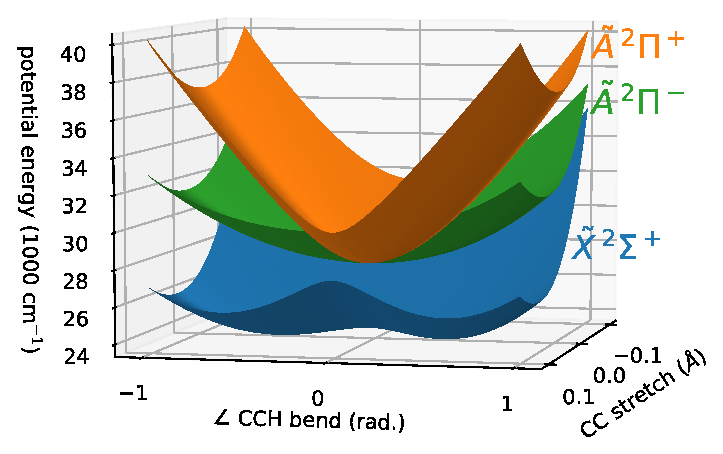
\includegraphics[width=0.5\textwidth]{figures/Fig2}
	\caption{Adiabatic potential energy surfaces of $\tilde{X}^2\Sigma^+$, $\tilde{A}^2\Pi^-$, and $\tilde{A}^2\Pi^+$ states, calculated using the parameters calculated by Tarroni and Carter~\cite{tar03}.}
	\label{fig:2}
\end{figure}

The adiabatic potential energy surfaces in Figure~\ref{fig:2} were evaluated from the variational parameters of Tarroni and Carter~\cite{tar03}, illustrating the loss of degeneracy for the doublet $^2\Pi$ surfaces, due to the Renner-Teller and pseudo Jahn-Teller interactions. This technique has been used to calculate a multitude of admixed vibronic levels. More than 100 possible C$_2$H vibronic states have been calculated, up to 10,000~cm$^{-1}$ above the $\tilde{X} ^2\Sigma^+$ origin. However, assigning experimental spectra has remained a challenge, partly due to the large number of calculated levels providing for multiple possible assignments for each experimentally observed transition.


\subsection{Coupling Calculations}
In order to guide spectral assignment of C$_2$H and future astronomical searches for other C$_n$H radicals, transition intensities are also needed. However, due to the strong vibronic coupling interactions, transition intensities can not be obtained via simple Franck-Condon calculations based on quantum chemistry methods. To account for these interactions, the photoelectron spectrum of the C$_2$H$^-$ anion is simulated using a quasidiabatic Hamiltonian of the type advocated by Koeppel, Domcke and Cederbaum (KDC).~\cite{kou84,dom81} In this approach, the Hamiltonian is represented in a basis of quasidiabatic (slowly varying) electronic  states for which the kinetic energy operator can be assumed diagonal.~\cite{pac93} For C$_2$H, the KDC Hamiltonian comprises three states - the two components of the $^2\Pi$ state and the ground $^2\Sigma^+$ state - and is then projected onto a vibrational basis, usually chosen as a direct product of harmonic oscillators. Diagonalization of the corresponding matrix yields the molecular states (which are given in terms of a Born-Huang expansion), and the squared projections of the corresponding eigenvectors onto the ground state of the anion yield the relative intensities. The latter is true only if the photodetachment cross sections for the $^2\Sigma^+$ and $^2\Pi$ states are assumed equal, but different cross sections of the two states can be incorporated by scaling the intensities of states according to their (vibronic) symmetry.~\cite{sta11} 

Details of the construction and parametrization of KDC Hamiltonians can be found elsewhere in the literature,~\cite{sta21,ich06,ich08,ich09,wei17} and the procedure followed will be discussed here only briefly. The present calculations use the so-called quadratic vibronic coupling (QVC) model.~\cite{ich06} For the system at hand, the QVC model Hamiltonian  assumes the following form

\begin{align}
H &= T_n1+V,\\
V &= \bordermatrix{ & X & A(a') & A(a'') \cr
	X &\substack{\Delta_0^X+F_1^Xq_1+F_3^Xq_3+\\ 
		\frac{1}{2} \sum_{ij}F^X_{ij}q_iq_j}& \lambda q_{2a} & \lambda q_{2b} \cr
	A(a') & \lambda q_{2a} & \substack{\Delta^A_0+F^A_1q_1+F^A_3q_3\\+\frac{1}{2}\sum_{ij}F^A_{ij}q_iq_j+\\\frac{1}{2}\eta(q_{2a}^2-q_{2b}^2)} & \eta q_{2a}q_{2b} \cr
	A(a'') & \lambda q_{2b} & \eta q_{2a}q_{2b} & \substack{\Delta_0^A+F_1^Aq_1+F_3^Aq_3\\+\frac{1}{2}\sum_{ij}F_{ij}^Aq_iq_j\\-\frac{1}{2}\eta(q_{2a}^2-q_{2b}^2) } } \qquad
\label{eq:calc1}
\end{align}

where the summations run over the dimensionless normal modes ($q_i$) that serve as the coordinate system for the problem.~\cite{sta21,car00} For convenience, the latter are chosen to be those of the anion, which considerably facilitates calculation of the spectral intensities.  In Eq.~(\ref{eq:calc1}), the diagonal terms of V (excluding those that carry the Renner-Teller coupling constant $\eta$) represent the quasidiabatic potential energy surfaces of the $^2\Sigma^+$ state, and the two components of the $^2\Pi$ state, chosen here as those in which the unpaired electron lies within or is perpendicular to an arbitrarily chosen plane, designated as A(a$'$) and A(a$''$), respectively. $\Delta_0^X$ is the separation of the anion and $^2\Sigma^+$ states at the origin of the coordinate system (the vertical electron detachment energy), and $\Delta_0^{A}$ is the gap between anion and $^2\Pi$ states at the same geometry.   

For the modes of $\sigma$ symmetry ($q_1$ and $q_3$), the diabatic forces ($F_i$) and force constants ($F_{ij}$) coincide with those of the adiabatic potential energy surfaces.   However, for the bending mode, the diabatic (F$_{22}$) and adiabatic (f$_{22}$) force constants differ, and the parametrization is somewhat more involved.   For each component of the $^2\Pi$ state, either the 2a or 2b component of the bending vibration will maintain the A$'$ electronic symmetry that is needed to couple with the $^2\Sigma^+$ state.  Designating these as 2a for the A(a$'$) state and 2b for the A(a$''$) state (as is implicit in Eq.~\ref{eq:calc1}), the diabatic force constants for the bending mode in the $^2\Sigma^+$ and $^2\Pi$ states can be written as 

\begin{align}
F_{22}^X &= f_{22}^X+\frac{2\lambda^2}{(\Delta_0^A-\Delta_0^X)}\\
F_{22}^A &= f_{2a2a}^{A(a')}-\frac{2\lambda^2}{(\Delta_0^A-\Delta_0^X)}-\eta
\label{eq:calc2}
\end{align}

where the Renner-Teller interaction strength ($\eta$) is determined from 

\begin{equation}
\eta = \frac{1}{2}\left[ f_{2a2a}^{A(a')}-f_{2b2b}^{A(a')}-\frac{2\lambda^2}{(\Delta_0^A-\Delta_0^X)}\right]
\label{eq:calc3}
\end{equation}

once the interstate coupling ($\lambda$ which is calculated analytically in this work, see below) is known.

When the potential in Eq.~(\ref{eq:calc1}) is diagonalized, the adiabatic states that are used for its parametrization are precisely recovered through terms second order in displacement. The linear diabatic coupling constants between the electronic states of interest were calculated analytically at the EOM-CCSD/ANO2 level of theory, using the CFOUR computational package~\cite{dev20} and the quasidiabatic ansatz of Ichino~\emph{et al.}~\cite{ich09} Briefly, the EOM procedure is used to operationally define quasidiabatic states (those that relax according to a well-behaved reference state wavefunction, which is that of the anion level) and the coupling constants are then evaluated as the first derivative of the off-diagonal elements of the electronic Hamiltonian in the basis defined by this representation. The diabatic force and coupling constants calculated to parametrize the KDC potential in Eq.~(\ref{eq:calc1}) were calculated at the CCSDT/ANO2 level of theory, and are presented in Table~\ref{tab:1}.


\begin{table}
	\caption{Parameters for the quasidiabatic Hamiltonian Eq.~(\ref{eq:calc1}) determined using CFOUR and the quasidiabatic ansatz. Units are in cm$^{-1}$.}
	\label{tab:1}

	\begin{tabular}{c | r r r r | r r r r} 
		\hline
		& \multicolumn{4}{c}{C2H} & \multicolumn{4}{c}{C2D}\\
		\hline
		& ~~Anion~~ & ~~$\tilde{X}^2\Sigma^+$~~ & ~~$\tilde{A}^2\Pi (a')$~~ & ~~$\tilde{A}^2\Pi (a'')$~~ & ~~Anion~~ & ~~$\tilde{X}^2\Sigma^+$~~ & ~~$\tilde{A}^2\Pi (a')$~~ & ~~$\tilde{A}^2\Pi (a'')$~  \\
		\hline
		$\Delta_0$ & 0& 22431.21&  26543.67& 26543.67& 0 & 22431.21& 26543.67& 26543.67 \\
		F$_1$ &  0& -211.28& 286.90& 286.90& 0& -596.04& 641.6& 641.6\\
		F$_3$ &  0& -1515.21&  1257.07& 1257.07& 0& -1401.53& 1115.17& 1115.17\\
		F$_{2a}$& 0 & 0& 0& 0& 0& 0& 0&0 \\
		F$_{2b}$&  0& 0& 0& 0& 0& 0& 0&0 \\
		F$_{11}$& 3424.32 &  3487.03& 3482.16& 3482.16& 2611.42&  2636.57& 2681.25& 2681.25\\
		F$_{13}$&  0 & -28.32& 31.46& 31.46& 0& -48.38& 55.40& 55.40\\
		F$_{33}$& 1894.71 & 1830.83& 2042.21& 2042.21& 1792.49&  1747.62& 1914.39& 1914.39\\
		f$_{22}$& 607.09&  87.57& -& -& 481.89&  120.09& -& -\\
		F$_{22}$& 607.09 & 770.78& -& -& 481.89& 620.70& -& -\\
		f$_{2a2a}$& - &- & 1883.48& 658.96& -& -& 1503.88& 473.55\\
		f$_{2b2b}$& - &- & 658.96& 1883.48& -& -& 473.55& 1503.88\\
		F$_{2a2a}$& -& -& 1200.27& 658.96& -& -& 1003.27& 473.55\\
		F$_{2b2b}$& -& -& 658.96& 1200.27& -& -& 473.55& 1003.27\\
		&&&&&&&& \\
		$\lambda$& & & -1185.26& & & & -1014.58& \\
		$\eta$ & & & -270.66& & & & -264.86& \\
		
	\end{tabular}
\end{table}

\subsection{Simulated Spectra}
The above method was employed to simulate the photoelectron spectrum of C$_2$H$^-$, with the calculated transitions shown in Figure~\ref{fig:3}(a) alongside the experimental data at 355~nm. Photoelectron spectra are simulated using the xsim package of CFOUR and the model Hamiltonian generated above. The Hamiltonian is diagonalised using the Lanczos algorithm, to calculate transition energies and intensities that map to the measured photoelectron spectrum.  
On the $\tilde{X} ^2\Sigma^+$ surface, below 3,600~cm$^{-1}$, there is excellent agreement in both the transition positions and intensities between the simulated and experimental spectra. This includes the HT coupled (2$^{n+1}$) transitions with $\Pi$ symmetry, which would normally be missing from a simulation using the standard \emph{ab-initio} approaches. 

The positions of the calculated levels for the $\tilde{A}^2\Pi$ state have been shifted by 1,220~cm$^{-1}$ to account for the EOMIP-CCSDT calculations overestimating the effective Term energy. The experimental data show that the electronic coupling interactions induce a splitting of the $\tilde{A} ^2\Pi$ state origin over 5 vibronic levels, spaced by $\sim 95~$cm$^{-1}$ ($a-e$). This splitting is also observed in the calculated spectrum, which reproduces the 5 prominent transitions in this region. The relative intensities between the calculated transitions are also in agreement with the experimental data. Peak $d$ is slightly overestimated in intensity, which may in part be due to the variation of photodetachment cross section near threshold, as described by the Wigner threshold law~\cite{wig48}. The simulated spectrum also slightly underestimates the splitting between the vibronic levels, which may be linked to the overestimation of the calculated gap between the $^2\Sigma$ and $^2\Pi$ surfaces.

\begin{figure}[th!]
	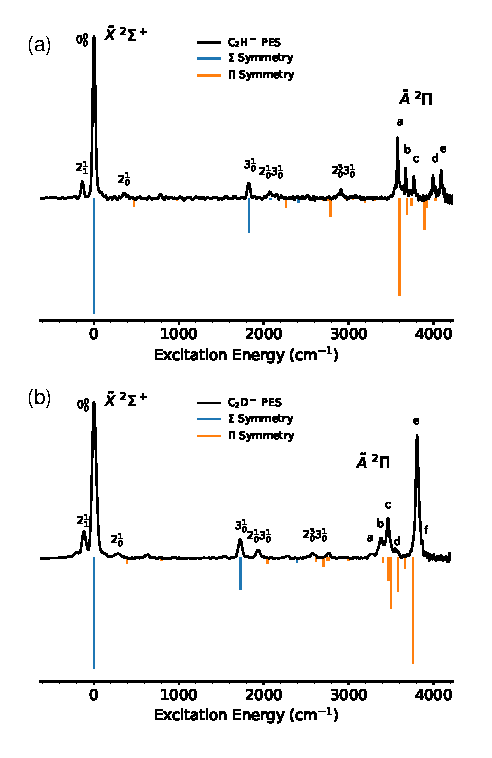
\includegraphics[width=0.6\textwidth]{figures/Fig3}
	\caption{(a) Experimental photoelectron spectrum of C$_2$H$^-$ at 355~nm, compared with the simulated spectrum, calculated using the quasidiabatic ansatz. Transitions with $\Sigma$ symmetry are shown in blue, and those with $\Pi$ symmetry are shown in orange. (b) Experimental photoelectron spectrum of C$_2$D$^-$ at 355~nm, compared to the simulated spectrum. The labelling of peaks near the $\tilde{A}$ origin correspond to transitions identified in Tables~S1 and~S2.}
	\label{fig:3}
\end{figure}

The photoelectron spectrum of C$_2$D$^-$ was also examined using the same approach, with the calculated transitions shown in Figure~\ref{fig:3}(b) alongside the 355~nm experimental data. Again, there is excellent agreement in the intensity and calculated positions of the transitions on the $\tilde{X} ^2\Sigma^+$ state surface, including the HT coupled levels. Near the $\tilde{A} ^2\Pi$ state origin, deuteration has a large impact on the experimental photoelectron spectrum. Instead of the 5 evenly split levels observed in C$_2$H, a single dominant peak ($e$) is now observed near $\sim3,845$~cm$^{-1}$ alongside a collection of weaker peaks ($a-d$) centred around 3,400~cm$^{-1}$. Based on the observed spin-orbit splitting measurements from rotationally resolved IR spectra~\cite{yan87,sch98,ste88}, peak $e$ is expected to have significant $\tilde{A} ^2\Pi$ character, with peaks $a-d$ commonly assigned to vibronic levels with predominantly HT coupled $\tilde{X} ^2\Sigma^+$ character~\cite{yan87,hsu95,chi99,wil11}. This suggests that deuteration effectively dampens the coupling interaction between the surfaces, as has been observed in the vinylidene photoelectron spectrum~\cite{dev17}.

The simulated spectrum reproduces the large change observed for the deuterated species. The calculated intensity pattern of the vibronic levels around the $\tilde{A} ^2\Pi$ origin also mirrors the experimental data, with a single intense transition observed near peak $e$, and 3 prominent transitions predicted around the experimental peaks $a-d$. The calculated splitting between the levels is also similar. 


To investigate the effects of coupling on the higher excited vibronic levels on the~$\tilde{A} ^2\Pi$ surface, the calculations were compared with the experimental photoelectron spectrum of C$_2$H$^-$ at 266~nm, as presented in Figure~\ref{fig:4}. Gaussian functions were fitted to the transitions from Figure~\ref{fig:3}(a) with a kinetic energy dependent FWHM of $\Delta\text{E}/\text{E} = 0.4\%$ ($\Gamma=55-30$~cm$^{-1}$) to match the lower resolution of the experimental data at high electron kinetic energies. Near 3,900~cm$^{-1}$ excitation energy the electronic origin of the $\tilde{A} ^2\Pi$ state is split over 5 vibronic levels, as has been discussed above. A similar effect is also observed for the $3^1_0$ band, which becomes split over 3 vibronic levels labelled $l$, $n$, and $o$. The calculated spectrum correctly predicts the position and intensity of peaks $n$ and $o$, but appears to strongly underestimate the intensity of peak $l$. Between the $0^0_0$ and $3^1_0$ bands a collection of weaker peaks are also observed ($f-k$). These are assigned to highly excited HT coupled $\tilde{X} ^2\Sigma^+$ transitions ($j,k$), admixed $\tilde{X}-\tilde{A}$ transitions ($h,i$) and pure $\tilde{X} ^2\Sigma^+$ transitions ($f$). Consequently, peak $f$ will possess $\Sigma$ symmetry, and should have a different anisotropy to all of the other dominant transitions above 3,800~cm$^{-1}$. The position and intensity of these highly-excited coupled transitions are well described by the simulated spectrum. 

\begin{figure}[th!]
	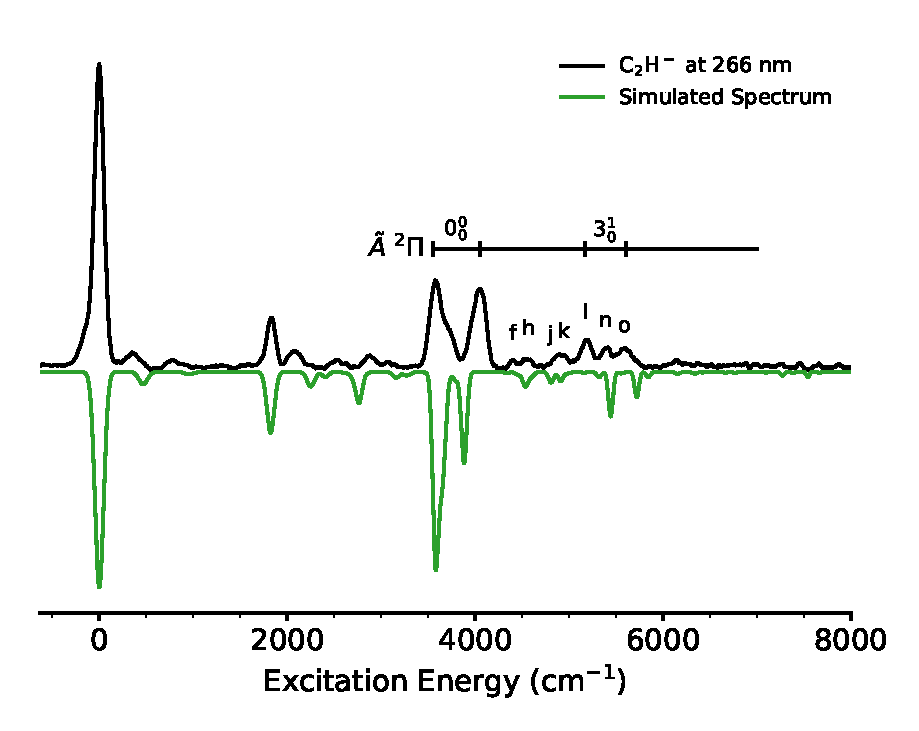
\includegraphics[width=0.6\textwidth]{figures/Fig4}
	\caption{Photoelectron spectrum of C$_2$H$^-$ at 266~nm, showing vibrationally excited $\tilde{A}$ state structure. The simulated spectrum, shown in green, is calculated using the quasidiabatic ansatz, and convolved with a Gaussian function with a kinetic energy dependent FWHM of $\Delta\text{E}/\text{E} = 0.4\%$ ($\Gamma=55-30$~cm$^{-1}$) to match the VMI resolution characteristics.}
	\label{fig:4}
\end{figure}

The results from Figures~\ref{fig:3} and~\ref{fig:4} confirm that the quasidiabatic approach is able to accurately describe the vibronic interactions between the $^2\Sigma^+$ and $^2\Pi$ surfaces, including deuteration effects. This validates the proposed vibronic interactions, and demonstrates how this method can be employed to decode and assign even complex spectra. While the present calculations invoke a high level of \emph{ab-initio} theory (EOM-CCSDT), the level of parametrization of the vibronic Hamiltonian is relatively simple (QVC model). The approach could be systematically improved with a more elaborate expansion, such as that used in Ref.~\onlinecite{sim12} for the NO$_3$ radical. Applying this approach to similar systems will produce reliable predictions for the position and intensity of dominant transitions, and help guide the search for these molecules in laboratory experiments and astronomical observations. 



\subsection{Photoelectron Angular Distributions}
Symmetry considerations may be employed to verify the spectral assignments from the calculations above. The quasidiabatic Hamiltonian approach is able to determine the symmetry of each individual vibronic state, either $\Sigma$ or $\Pi$, which may be compared directly to the observed anisotropy of each transition. The velocity-map images from this work (Fig~\ref{fig:1}) were obtained using a linearly polarized detachment laser. Therefore, the differential cross section of emitted electrons is given by,  
\begin{equation}
\frac{\text{d}\sigma}{\text{d}\Omega}=\frac{\sigma_{\text{total}}}{4\pi}[1+\beta P_{2}(\cos\theta)],
\label{eq:beta1}
\end{equation}
where $\theta$ is the angle between the ejected electron and the (vertical) 
laser polarization, and $P_2$ is the second-order Legendre polynomial. The anisotropy parameter $\beta$ provides a quantitative measure of the electron anisotropy, which ranges from -1 to +2, the limits representing purely perpendicular and parallel transitions respectively. Through conservation of angular momentum, $\beta$ may be described in terms of the detachment partial waves, which are linked to the symmetry of the state accessed by photodetachment. This is discussed in detail elsewhere\cite{khu14,law19}, and is only briefly described for the case of C$_2$H$^-$ here. 

Photodetachment to the ground state of C$_2$H $(\tilde{X}\,^2\Sigma^+)$ involves ejecting an electron from an $s-$like $\sigma$ orbital (approximately $5\sigma_g$ in symmetry character), whereas detachment to the excited $\tilde{A}\,^2\Pi$ state occurs from a $p-$like $\pi$ orbital (approximately $1\pi_u$ in character)~\cite{gul21}. Therefore, the electron anisotropies may be described using the mixed $s-p$ model\cite{khu14},
\begin{equation}
\beta_{sp}(\epsilon) = \frac{2(1-\gamma_p)B_1\epsilon + \gamma_p(2A_1^2\epsilon^2-4A_1\epsilon\cos\delta_{2,0})}
{(1-\gamma_p)B_1\epsilon+\gamma_p(1+2A_1^2\epsilon^2)}
\label{eq:beta-sp}
\end{equation}
where $\epsilon$ is the electron kinetic energy and $\gamma_p$ is the fraction of $p$ character of the detachment orbital described as,
\begin{equation}
|\psi\rangle = \sqrt{1-\gamma_p}|s\rangle + \sqrt{\gamma_p}|p\rangle.
\end{equation}
$A_1$ and $B_1$ in Eq.~(\ref{eq:beta-sp}) are the generalised Hanstorp~\cite{han89} coefficients describing the assumed Wigner-like~\cite{wig48} relative scalings of the radial transition dipole matrix elements for different allowed detachment channels. Specifically, $A_1\epsilon$ describes the energy-dependent ratio of the $p\rightarrow d$ and $p\rightarrow s$ transition amplitudes, while $B_1\epsilon$ corresponds to the $s\rightarrow p$ and $p\rightarrow s$ cross-section ratio~\cite{khu14}. It can be shown that under certain approximations $B_1/A_1 = 8/3$~\cite{san13}. Finally, $\delta_{2,0}$ in Eq.~(\ref{eq:beta-sp}) is the phase shift between the $s$ and $d$ partial waves, which in most cases of anion photodetachment is assumed to be small, corresponding to $\cos\delta_{2,0}\approx1$.

From Eq.~(\ref{eq:beta-sp}) it can be seen that detachment from a pure $s$ orbital ($\gamma_p=0$) will have a positive anisotropy ($\beta = +2$), whereas detachment from a pure $p$ orbital ($\gamma_p=1$) will have a negative anisotropy for electron kinetic energies $\epsilon < 2/A_1$. Therefore, measuring the anisotropy can help determine the electronic character of each individual transition, which may be compared to the calculated symmetries in Figure~\ref{fig:3}. Anisotropy parameters were measured over a range of detachment wavelengths for prominent transitions in the C$_2$H$^-$ photoelectron spectra, and are presented in Figure~\ref{fig:5}. Fitting Eq.~(\ref{eq:beta-sp}) to the anisotropy parameters from $^2\Pi$ state detachment, with $\gamma_p = 0.9$ produces a Hanstorp coefficient of $A_1=0.66(4)~$eV$^{-1}$.


\begin{figure}[th!]
	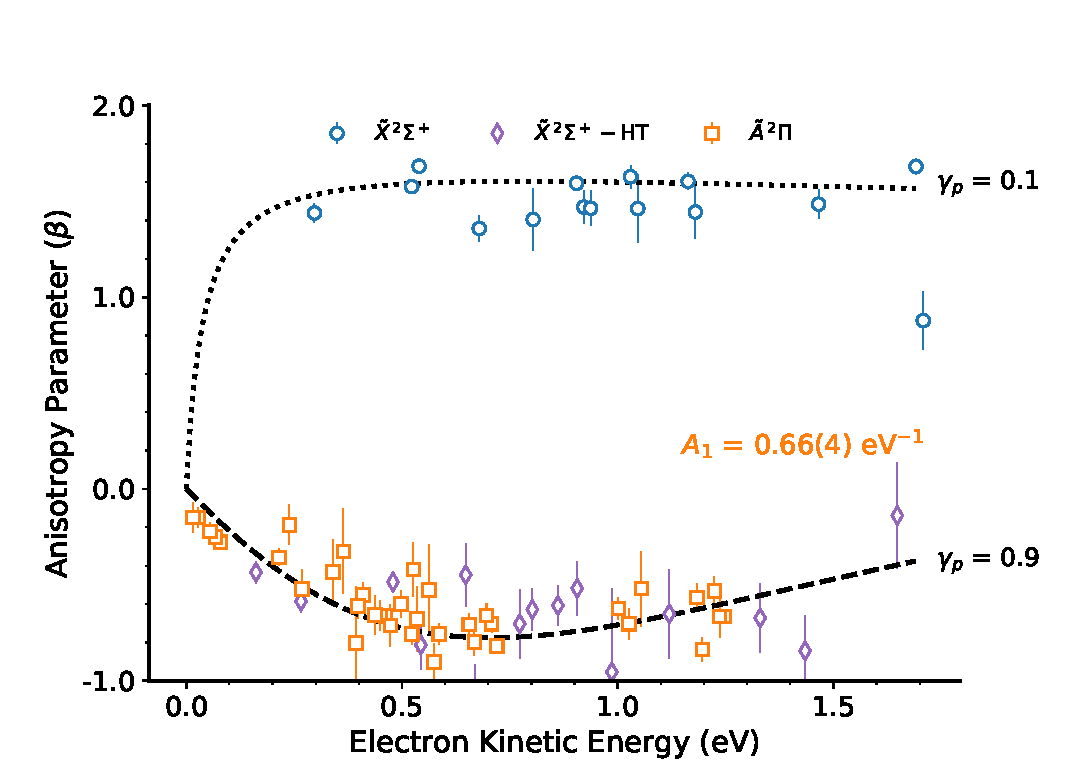
\includegraphics[width=0.5\textwidth]{figures/Fig5}
	\caption{Photoelectron anisotropy parameters, measured for each resolved C$_2$H$^-$ transition, across a range of detachment wavelengths. Allowed ground state transitions $\tilde{X}^2\Sigma^+$ are shown in orange, Herzberg-Teller coupled transitions are shown in purple, and excited state transitions $\tilde{A} ^2\Pi$ are shown in blue. Anisotropy curves for a mixed-$sp$ model (Eq.~\ref{eq:beta-sp}) are shown for $\gamma_p=0.1$ and $\gamma_p=0.9$.}
	\label{fig:5}
\end{figure}

The sign $(+/-)$ of $\beta$ can be used to assign each accessed vibronic level to either the $^2\Sigma^+$ or $^2\Pi$ vibronic symmetry respectively. This is particularly useful around the $\tilde{A} ^2\Pi$ origin, where the two states overlap. It is important to note that the HT coupled transitions on the $\tilde{X} ^2\Sigma^+$ surface have negative anisotropies and $\Pi$ symmetry. 

A plot of the anisotropy parameters for C$_2$H$^-$ detachment at 300~nm, represented as $\beta\times I$, is presented in Figure~\ref{fig:6}, alongside the photoelectron spectrum. Plotting $\beta\times I$ allows the sign $(+/-)$ of each individual transition to be easily identified, even for partially resolved peaks. All of the transitions above the $\tilde{A} ^2\Pi$ origin have a negative anisotropy parameter, except for peak $f$, which was not assigned in previous experiments. The positive anisotropy supports our assignment of this peak to the excited $\Sigma$ transition $\tilde{X}(0,6,1$), where $\tilde{X}(v_1,v_2,v_3)$. The nearby peaks $h$ and $i$  are assigned to the admixed $\Pi$ transitions $\tilde{X}(0,3,2)\tilde{A}(0,0,0)$ and $\tilde{X}(0,7,1)\tilde{A}(0,1,0)$, in agreement with previous assignments~\cite{zho07,tar03}. Peak $j$ was tentatively assigned to the $\Sigma$ transition $\tilde{X}(1,4,0$) previously~\cite{zho07}, however Figure~\ref{fig:6} shows peak $j$ has $\Pi$ symmetry. Therefore, we assign $j$ to the excited HT coupled $\Pi$ transition $\tilde{X}(0,7,1)$. The other dominant peaks in this region, $l$, $n$, and $o$, represent admixed $\Pi$ transitions involving the $\tilde{A}(0,0,1)$ vibrational level of the excited state. The complete assignments for all resolved peaks in the C$_2$H$^-$ and C$_2$D$^-$ photoelectron spectra from this work are presented in the Supplementary Materials Table~S1. Transition assignments are based on a combination of the previous works of Tarroni and Carter~\cite{tar03} and Zhou~\emph{et al.}~\cite{zho07}, the transition position and symmetry outputs from the QVC calculations (Fig.~\ref{fig:3}), and the experimental electron anisotropies which define the vibronic symmetry.

\begin{figure}[th!]
	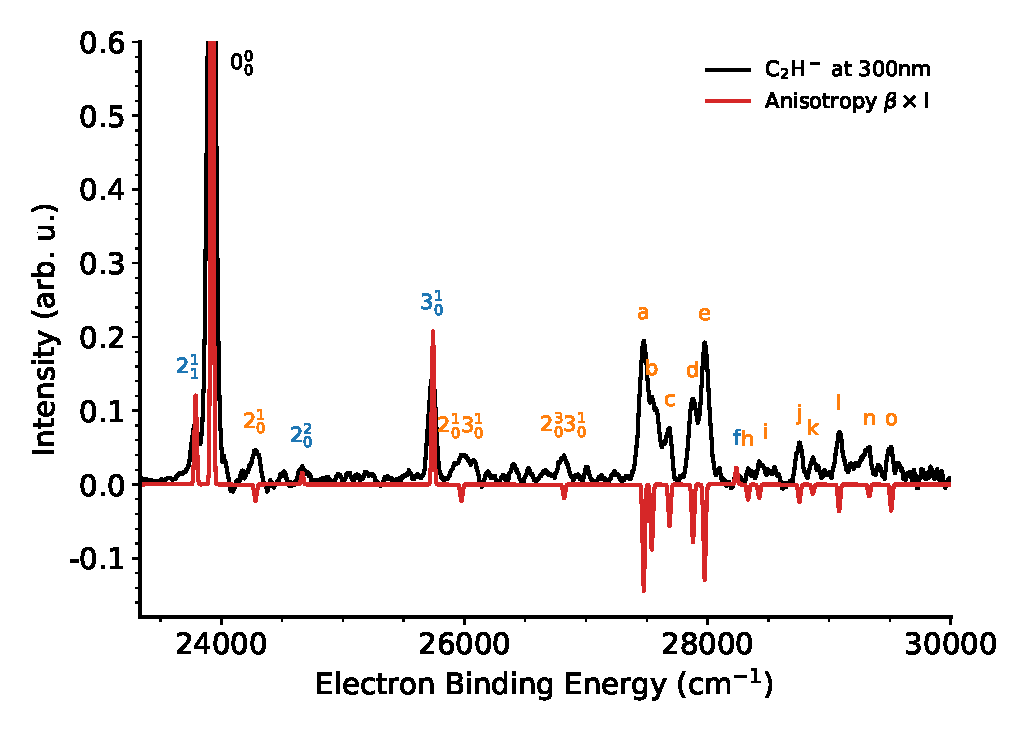
\includegraphics[width=0.6\textwidth]{figures/Fig6}
	\caption{Photoelectron spectrum of C$_2$H$^-$ at 300~nm, compared to anisotropy measurements, presented as $\beta\times I$. For each resolved transition the anisotropy parameter was determined from Eq.~(\ref{eq:beta1}) and multiplied by the corresponding photoelectron intensity. This allows for the sign $(+/-)$ of each transitions to be readily determined.}
	\label{fig:6}
\end{figure}

This result demonstrates how experimental anisotropies and calculated transition intensities can be combined to help assign and understand vibronically coupled spectra. This is particularly useful in spectral regions where there are a large number of potential vibronic transitions, making definitive assignments based on energetics alone difficult.



\section{Conclusions} 
High-resolution photoelectron images of C$_2$H$^-$ and C$_2$D$^-$ were recorded at a range of wavelengths, to investigate vibronic coupling effects in the simplest C$_{2n}$H carbon monohydride chain. The interplay of pseudo Jahn-Teller and Renner Teller coupling between the close lying $\tilde{X}^2\Sigma^+$ and $\tilde{A}^2\Pi$ states results in a complex vibronic spectrum near the $\tilde{A}$ state surface, with the electronic origin split over multiple admixed levels. By transforming to a quasidiabatic representation, the effect of these coupling interactions may be accurately simulated. A KDC Hamiltonian was constructed, and parametrised using the high-level EOM-CCSDT quantum chemical approach and the quasidiabatic ansatz. The resulting simulated photoelectron spectra of C$_2$H$^-$ and C$_2$D$^-$ resemble the experimental data, particularly in the complex energy region of the $\tilde{A}$ state origin. Photoelectron anisotropy parameters were also measured for dominant transitions, at a range of wavelengths. The sign $(+/-)$ of the anisotropy parameter, when compared to the calculated vibronic symmetry, allowed even weak or partially resolved transitions to be assigned.

The excellent agreement between the experimental and calculated spectra in this work
demonstrates that electronic spectra complicated by vibronic coupling effects may still be accurately simulated using a quasidiabatic treatment, as parametrised by appropriate quantum chemical methodology. This approach may be applied to larger, less well known, C$_{2n}$H species, which may help guide the search for these molecules in astronomical studies, and help identify potential DIB carriers. It is especially encouraging that the fairly modest parametrisation used here works so well for C$_2$H, as this bodes well for its extension to larger systems.


\section*{Supplementary Materials}
See supplementary material for the complete list of C$_2$H and C$_2$D photoelectron transitions and assignments.


\begin{acknowledgments}
	This research was supported by the Australian Research Council Discovery
	Project Grants DP160102585 and DP190103151.  
\end{acknowledgments}

\section*{Data Availability}
The data that support the findings of this study are available from the corresponding author upon reasonable request.

\bibliography{Laws_C2H}

\end{document}
%
% ****** End of file aiptemplate.tex ******